\documentclass[twoside, 10pt]{article}

\usepackage{geometry}
\geometry{outer=3em, inner=2.2cm, top=6em, bottom=4em, headheight=\paperheight}
\usepackage[export]{adjustbox}
\usepackage{array}
\usepackage{amsmath}
\usepackage{amsfonts}
\usepackage{fancyhdr}
\pagestyle{fancy}
\fancyhf{}
\lhead{Algebra II - BASE}
\chead{Function Composition}
\rhead{Reference, Page \thepage}
\usepackage{lastpage}
\usepackage{xcolor}
\usepackage{enumitem}
\usepackage{pifont}
\usepackage{graphicx}
\graphicspath{{../img}}
\usepackage{pgfplots}
\pgfplotsset{compat=1.18}
\usepackage{tabularx}
\usepackage{tikz}
\usetikzlibrary{patterns}

\newcommand{\R}{\mathbb R}
\newcommand{\e}{{\rm e}}
\newcommand{\pobr}[1]{\left\langle#1\right\rangle}
\newcommand{\norm}[1]{\lVert #1 \rVert}
\newcommand{\abs}[1]{\lvert #1 \rvert}

\DeclareMathOperator{\xd}{d\!}
\DeclareMathOperator{\proj}{proj}

\title{}
\date{}

\begin{document}
\begin{enumerate}
\item {\bf Evaluate a function.}
\begin{enumerate}
\item
To evaluate a {\bf function given by an algebraic formula}, you just need to replace the variable of the function by the input subject. For example, if \[(x) = x^2 - x,\]
then 
\[
 f(2) = (2)^2 -(2) = 4 - 2 = 2,\quad f(10) = (10)^2 - (10) = 100 - 10 = 90.
\]
The input value, namely, what you plug in, can be a number, or other algebraic expressions. For example,
\[
f(a) = a^2 - a,\quad f(x+1) = (x+1)^2 - (x+1)
\]

\item To evaluate a {\bf function given by a table}, you just need to look for the output value in the same column as the input value. For example,
\begin{center}
\renewcommand{\arraystretch}{2}
\begin{tabular}{|c|c|c|c|}
\hline
$x$ & 2&4&9\\
\hline
$f(x)$ &3&-1&0\\
\hline
\end{tabular}
\[
f(2) = 3,\quad f(4) = -1,\quad f(0) = \text{undefined}
\]
\end{center}
\item To evaluate a {\bf function given by a graph}, you just need to look for the point on the graph with the input value as the $x$-coordinate, then read the $y$-coordinate. For example,
\begin{center}

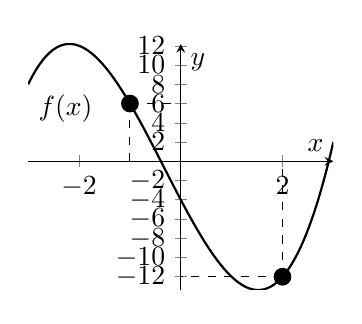
\begin{tikzpicture}
\begin{axis}[
xlabel={$x$},
ylabel={$y$},
axis lines=middle,
domain=-3:3,
samples=200,
ytick distance = 2,
width=.45\textwidth
]
\addplot[thick]{x^3 +x^2 -10* x-4} node[pos=0, below right]{$f(x)$};
\draw[fill=black] (-1, 6) circle (3pt);
\draw[dashed] (-1,6) -- (-1,0);
\draw[dashed] (-1,6) -- (0,6);
\draw[fill=black] (2,-12) circle (3pt);
\draw[dashed] (2,-12) -- (2,0);
\draw[dashed] (2,-12) -- (0,-12);
\end{axis}
\end{tikzpicture}
\end{center}
\[
f(-1) = 6,\quad f(2) = -12
\]
\end{enumerate}
\end{enumerate}
\end{document}